\section{Results}

\subsection{Range and Stopping Power}

\begin{figure}
\centering
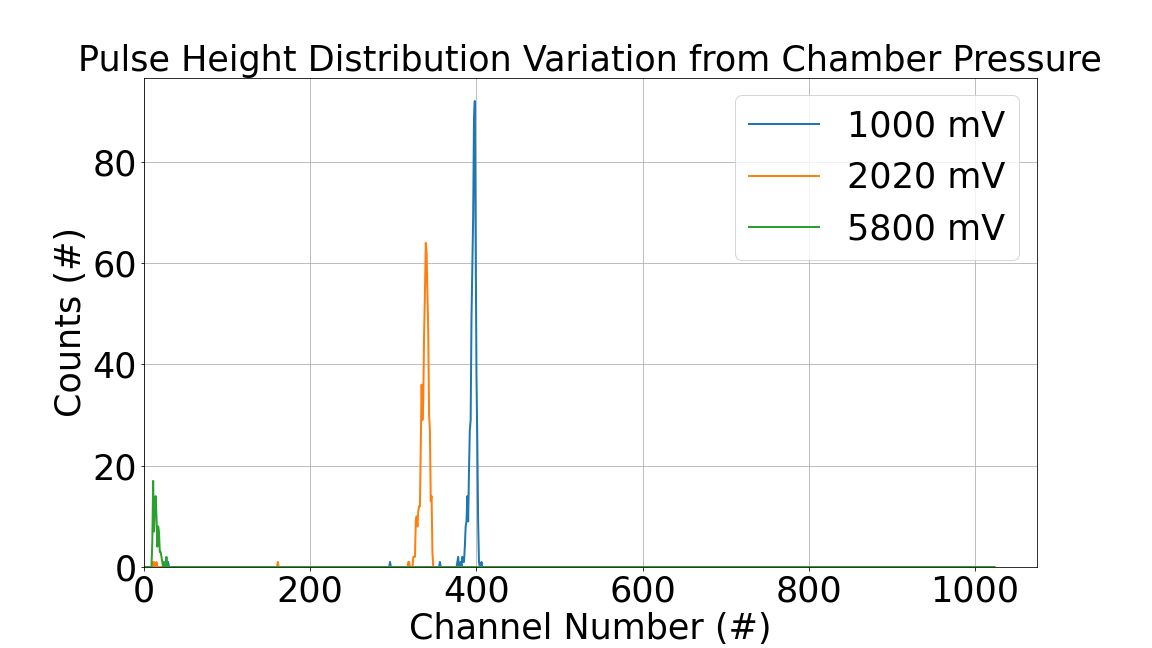
\includegraphics[scale=0.3]{variation.png}
\caption{Demonstration of the variation in pulse height distribution of $\alpha$ particles from ${}^{241}Am$. Distributions are labelled by the reading measured from the voltmeter pressure sensor. This voltage is linearly proportional to the actual pressure in the chamber. Not only does the position of the energy peak change with pressure but also the magnitude of the peak.}
\label{fig:variation}
\end{figure}

It is first important to demonstrate the ability of this experimental setup to vary peak energy position with pressure. This can be demonstrated by plotting several sample distributions at varying pressure values, as seen in Fig. \ref{fig:variation}. Each distribution is labelled by the voltage reading of the pressure sensor, but this is just a proxy of pressure and can proportionally represent the chamber’s pressure. Clearly the peak position varies not only in position but in magnitude. This shows that the pulse height distribution can be varied with pressure and thus a range can be measured.

\begin{figure}
\centering
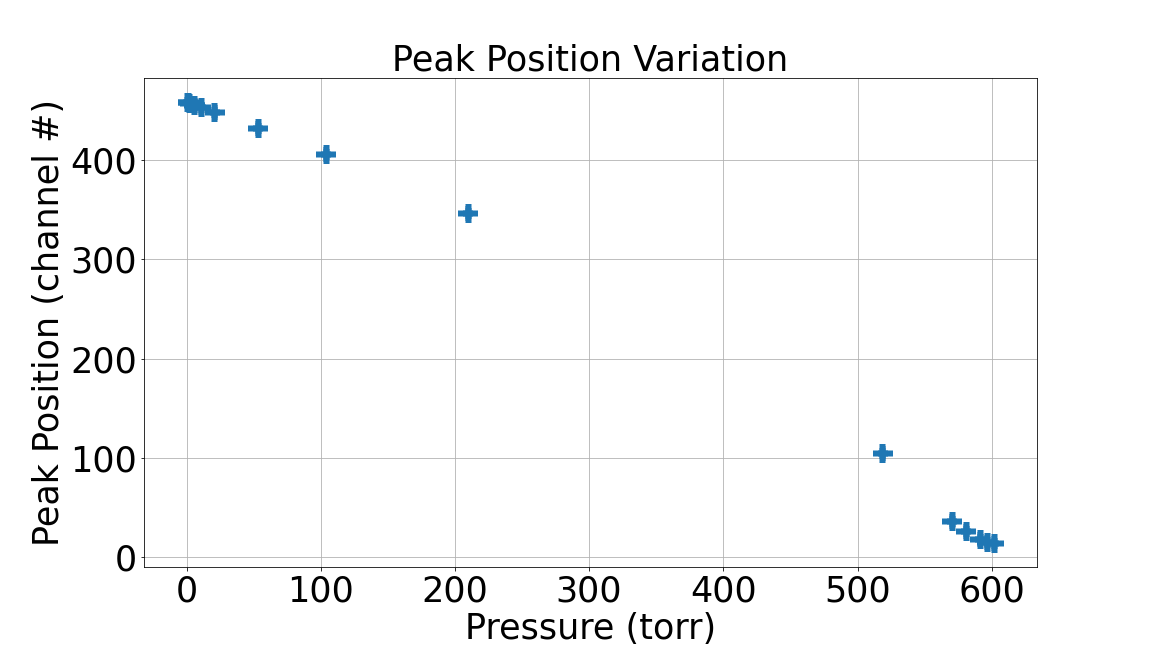
\includegraphics[width=\textwidth]{peak_position.png}
\caption{The center channel of the peak energy distribution is plotted as a function of pressure, listed in torr. The pressure is interpreted from the linearly proportional voltage reading in the experimental setup. Uncertainties, though small, are reported in the plot. These two parameters seem to be inversely proportional.}
\label{fig:peak-position}
\end{figure}

At atmospheric pressure (760 torr), the voltmeter read 7330 mV. This proportionality can be applied for samples taken over a wide range of pressure values and the channel number of the $\alpha$ peak position can be recorded. This relationship is plotted in Fig. \ref{fig:peak-position}. An effective distance, which is a way of describing the absorbing material’s thickness, can be calculated using the definition:

\begin{equation}
d_{\mathrm{eff}} = \frac{1}{\rho_{\mathrm{STP}}} \frac{P(MW)_{\mathrm{air}}}{RT}d
\end{equation}

Here $P$ is the pressure in Pascals, $\rho$ the absorber density, $d$ the fixed distance between the sample and the detector, $MW$ the molecular weight of the absorbing material, $T$ the temperature in Kelvin, and $R$ the universal gas constant. A mean energy can also be obtained from the center channel of the peak. If the lowest pressure reading is assumed to maintain the full $\alpha$ energy (5.486 MeV), and the trend is assumed to be linear, then the mean energy at each pressure reading can be proportionally calculated as well. These two parameters are plotted in Fig. \ref{fig:mean-energy}. Note that the uncertainty in the pressure reading is approximated at 2 torr. Since the relationship between effective distance and pressure is linear, the uncertainty in effective distance is linearly scaled (reflected in the plot). Likewise, the uncertainty in the peak channel is approximated at 2 channels and the uncertainty in mean energy is linearly scaled.

\begin{figure}
\centering
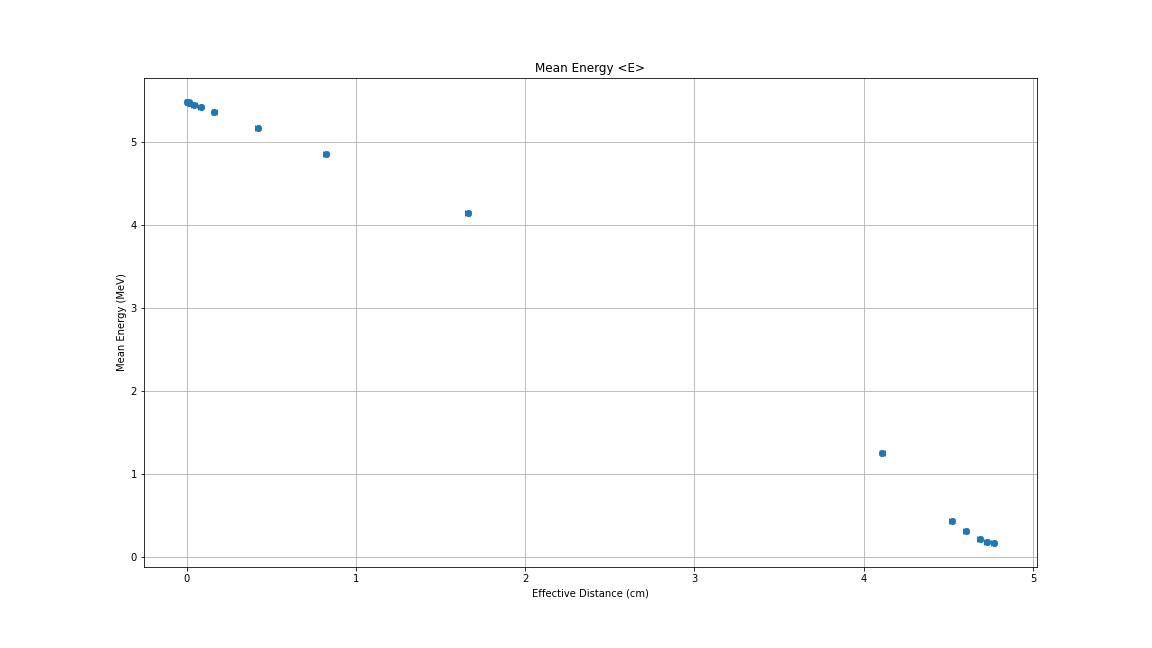
\includegraphics[width=\textwidth]{mean_energy.png}
\caption{This plots the mean energy in the peak distribution as a function of effective distance. Effective distance is a way of representing the thickness of the absorbing material, calculated from the chamber’s pressure. Mean energy is directly translated from the center channel number of the peak distribution recorded. Mean energy and center channel number are assumed to be linearly proportional where the lowest pressure recorded maintains the full energy of the $\alpha$ particles emitted: 5.486 MeV.}
\label{fig:mean-energy}
\end{figure}

 A mean stopping power ($-\frac{dE}{dx}$) can be inferred by diving the mean energy by the effective distance. This relationship can then be plotted as a function of the mean energy in Fig. \ref{fig:stopping-power}. The uncertainty in this stopping power can calculated using the error propagation of the uncertainty between the effective distance and the mean energy \cite{taylor}. Notice how the uncertainty increases dramatically at the very end of the curve because the exponential rise is so large. This acts as a wall for the travelling particle and an indication of a stopping range.

 \begin{figure}
 \centering
 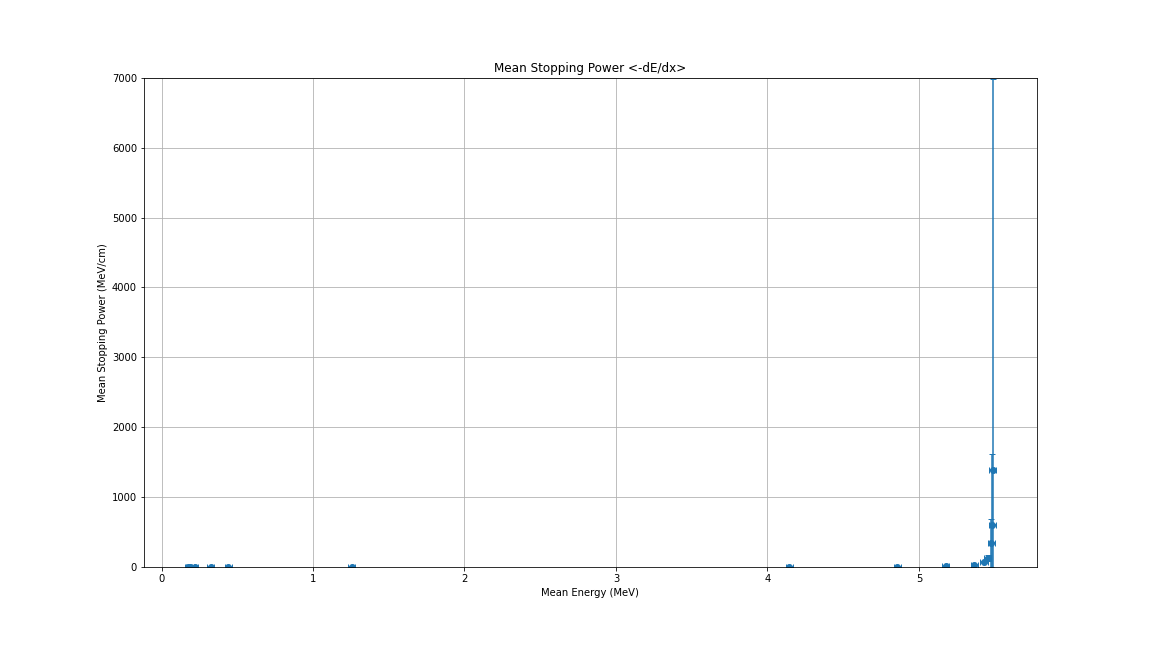
\includegraphics[width=\textwidth]{stopping_power.png}
 \caption{Mean stopping power (the mean energy per unit of effective distance) is plotted as a function of mean energy. Mean stopping power’s uncertainty is calculated from error propagation of its two dependent variables: mean energy and effective distance. Note how the uncertainty increases rapidly at high mean energy where the relationship exponential rises. This is representative of a stopping range where the stopping power increases significantly and the $\alpha$ particles are unable to move past.}
 \label{fig:stopping-power}
 \end{figure}

The range can more clearly be seen by taking the detector count rate of the energy peak as a function of effective distance. The MCA calculates the net counts under the peak energy and is then normalized by the 60 s integration time in the experiment. The uncertainty in this measurement is just the standard statistical uncertainty ($\sqrt{N}$) in a measurement of this kind. This relationship is illustrated in Fig. \ref{fig:count-rate}. Clearly there is some effective distance at which the $\alpha$ particles cannot reach before being stopped/absorbed. A linear interpolation of the end of this range results in $R_{\alpha}$ = 4.81 $\pm$ 0.43 cm. The linear interpolation was made using to points on the linear end of the curve and extrapolated to a count rate of 0. The uncertainty was calculated using error propagation (each parameter in the linear interpolation has some uncertainty and that error propagates to the ultimate answer for the range).

\begin{figure}
\centering
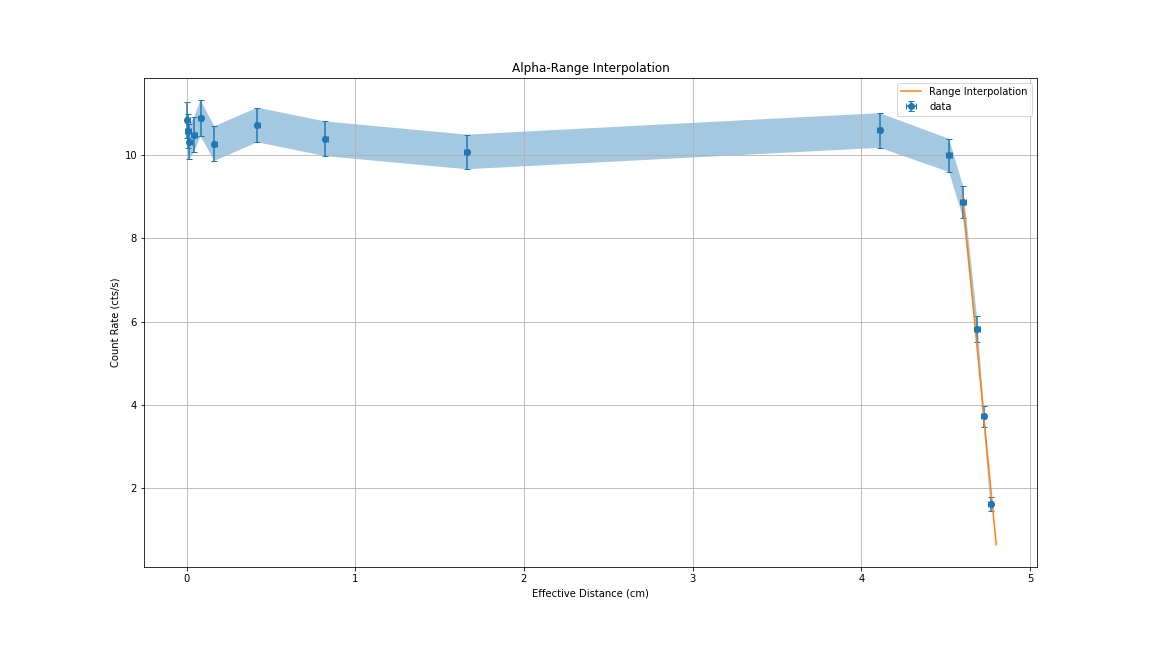
\includegraphics[width=\textwidth]{count_rate.png}
\caption{The detector count rate of the $\alpha$ energy peak as a function of effective distance. This shows that after some amount of absorbing material, $\alpha$ particles are not able to continue travelling and are stopped/absorbed. The end of this distribution can be interpreted as the range of $\alpha$ particles in this medium at the characteristic energy. It can be measured by interpolating the linear portion of the distribution and extrapolating that value to 0 count rates.}
\label{fig:count-rate}
\end{figure}

\subsection{Mass Attenuation Coefficient}

\begin{figure}
\centering
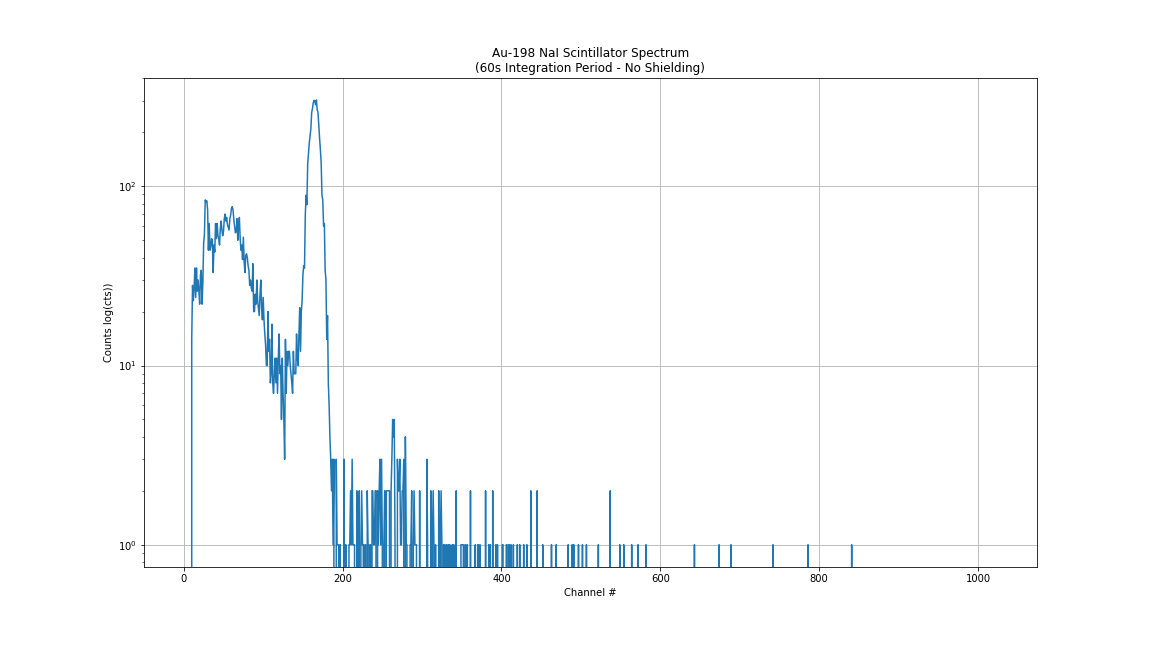
\includegraphics[width=\textwidth]{au198_spectrum.png}
\caption{Representative ${}^{198}Au$ energy spectrum plotted in a semi-logarithmic (y) scale. While this spectrum has not been energy calibrated, the 411.8 keV photopeak is clearly visible and intense enough to record peak statistics.}
\label{fig:au198-spectrum}
\end{figure}

First the characteristic gamma spectrum can be plotted as received from the NaI scintillator in Fig. \ref{fig:au198-spectrum}. This spectrum was collected during a 60 s integration period with no shielding of the ${}^{198}Au$ source. Notice the signature 411.8 keV photopeak clearly visible in the distribution. The intensity of this peak can be measured and tracked as shielding thickness is varied to find a relationship and extract the attenuation coefficient. Before that, the background count rate needs to be determined and removed from the gross peak counts. The background was measured for 60 s with the source plugged and is plotted in Fig. \ref{fig:background}. This background was assumed to be linearly related to the thickness of the shielding material and a linear relationship was extrapolated. This was applied to data collected for both aluminum and lead shielding and a net count rate was calculated.

\begin{figure}
\centering
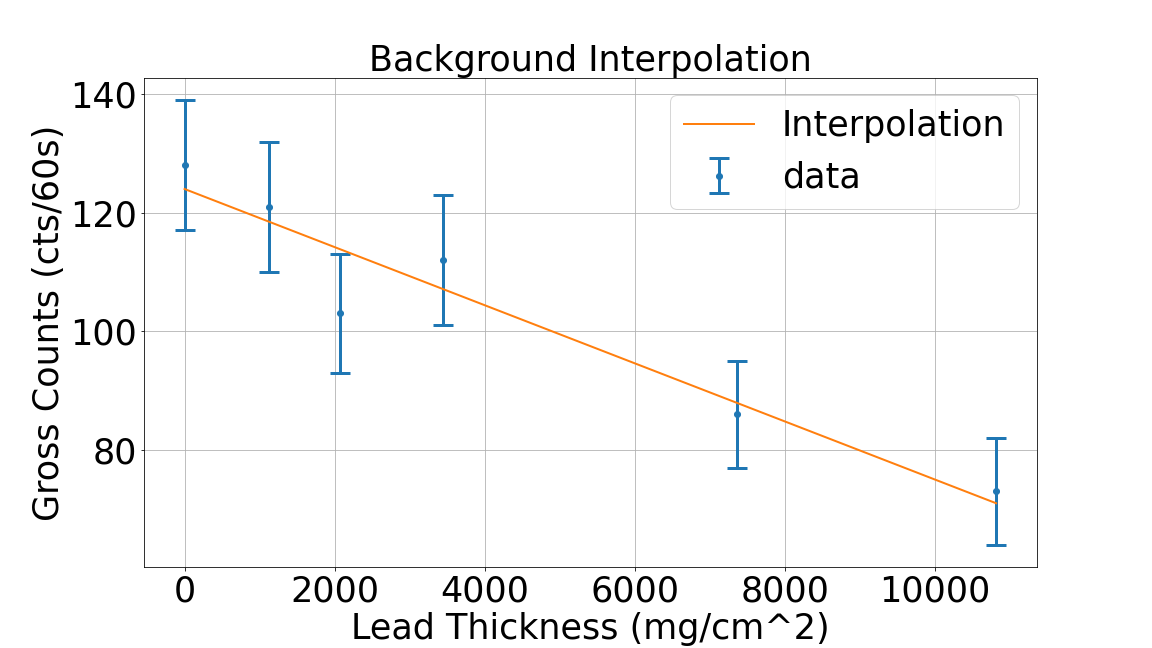
\includegraphics[width=\textwidth]{background.png}
\caption{The background radiation detected in the NaI scintillator is plotted here. This data is collected by recording measurements at varying lead shielding thickness with the radiation source plugged. The background is assumed to be linear in regard to the shielding thickness and a linear relationship is plotted and interpolated.}
\label{fig:background}
\end{figure}

\begin{figure}
\centering
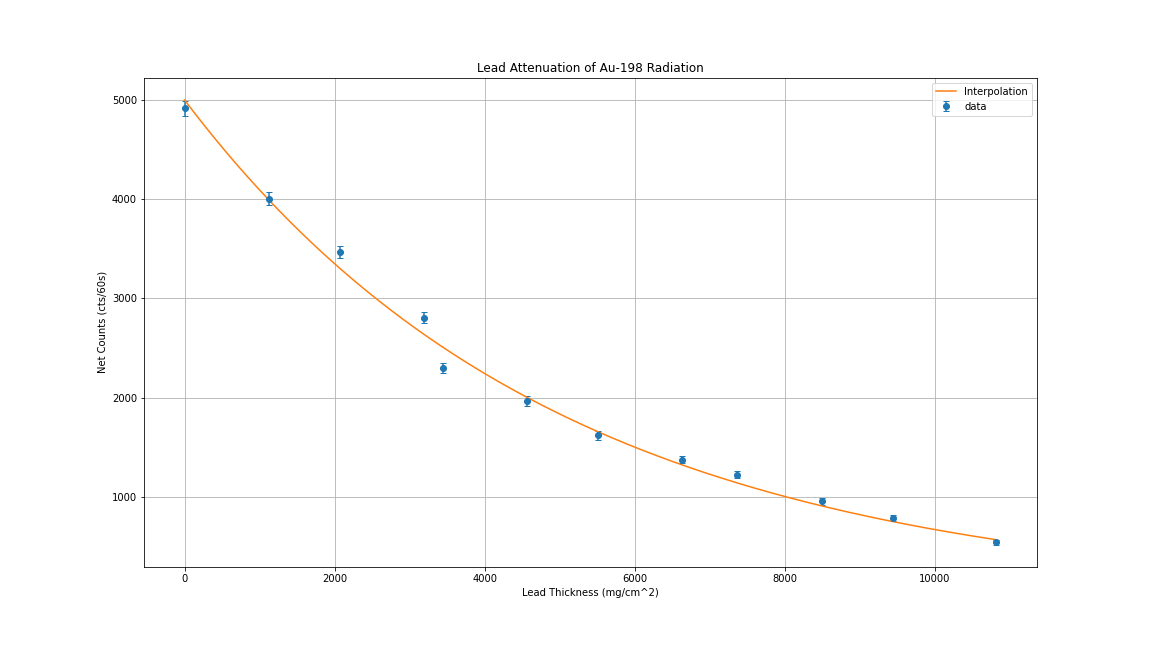
\includegraphics[width=\textwidth]{Pb.png}
\caption{The attenuation of gamma radiation is plotted for different thicknesses of lead. The data exhibits an exponential decay behavior indicative of gamma attenuation. This data can be fitted to a characteristic function and the mass attenuation coefficient can be extracted from the fit.}
\label{fig:Pb}
\end{figure}

Lead attenuation is plotted in Fig. \ref{fig:Pb}. The uncertainty in this data is quantified as the error propagation of statistical uncertainty in the gross counts and uncertainty related to the linear coefficients from the background interpolation. This data exhibits an exponential decay behavior and a fitted line is also plotted. The parameters of this fit can be extracted as the parameters from Eq. \ref{eq:decay}. This results in a mass attenuation coefficient of $(\frac{\mu}{\rho})$ = 1.98 $\pm$ 0.04 $\times 10^{-4}$ $(\frac{mg}{cm^2})^{-1}$. The uncertainty in this coefficient was extracted from the fit using Microsoft Excel’s $\mathrm{LINEST}$ function, which extracts standard deviations from fits (which are calculated using a least squares method). Similarly, the relationship for aluminum attenuation can be plotted in Fig. \ref{fig:Al}. Again, the data is fitted to an exponential decay and the coefficient (including its uncertainty) is extracted as $(\frac{\mu}{\rho})$ = 8.72 $\pm$ 0.24 $\times 10^{-5}$ $(\frac{mg}{cm^2})^{-1}$.

\begin{figure}
\centering
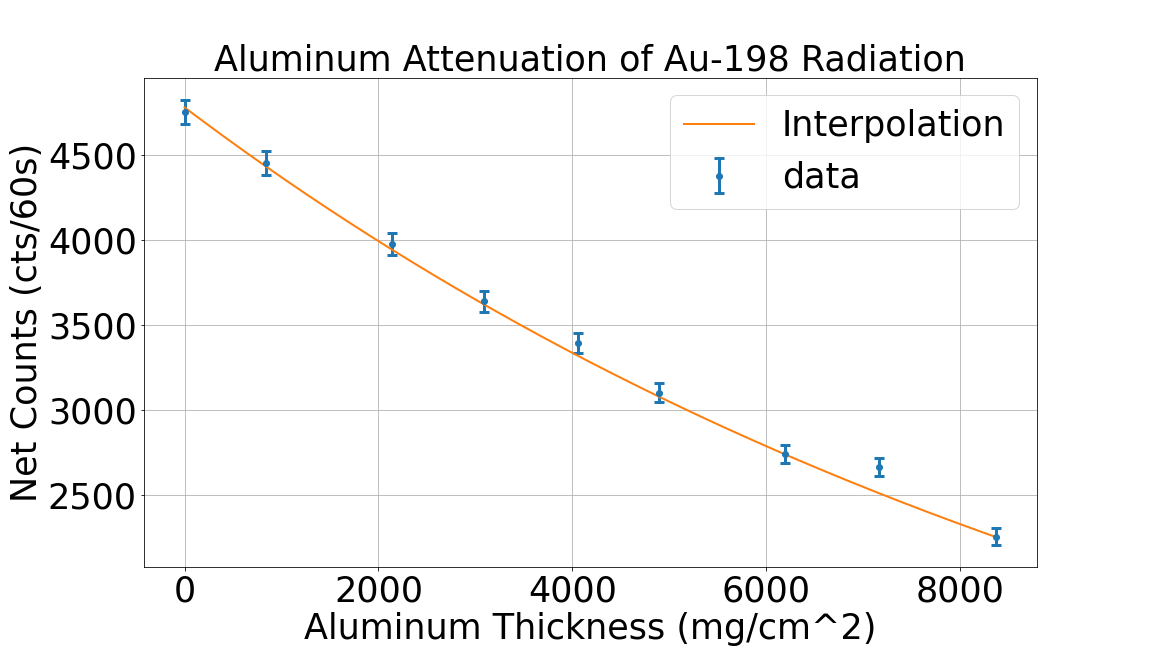
\includegraphics[width=\textwidth]{Al.png}
\caption{The attenuation of gamma radiation is plotted for different thicknesses of aluminum. The data exhibits an exponential decay behavior indicative of gamma attenuation. This data can be fitted to a characteristic function and the mass attenuation coefficient can be extracted from the fit.}
\label{fig:Al}
\end{figure}
